\section{Benchmarking the Implementation Schemes}
\label{bench}
The main problem that we encountered when implementing cooperative scheduling was saving the context of an execution and resuming from that context. To do this in Java using threads and context switches heavily limits the application to the number of native threads that can be created. To measure the improvement provided by Java 8 features, we benchmark a simple example that is illustrated in Listing \ref{absex}. This example creates an Actor of type "A" and sends a large number of messages to it to execute a method \lstinline|recursive_m(5,id)|. This method creates a call chain of size 5 before sending an asynchronous message to itself to execute a basic method \lstinline|compute()| and awaits on its result.

%In the
%example we have one actor containing an which receives a large
%number of messages stored in its queue. This message recursively calls
%a function that creates a stack frame after which a message is
%sent to a different Actor to run in parallel a function that computes a large number of trigonometric operations . The object is then suspended to await the
%result of this function, resulting in the requirement to save the stack frame in order to allow the next message from the queue to run
%on the actor. We varied the total number
%of messages in the object's queue to compare performance between a trivial thread based approach and our optimized solution in the Java backend for ABS. 

%\begin{figure}
%	\label{sf}
%	\centering
%	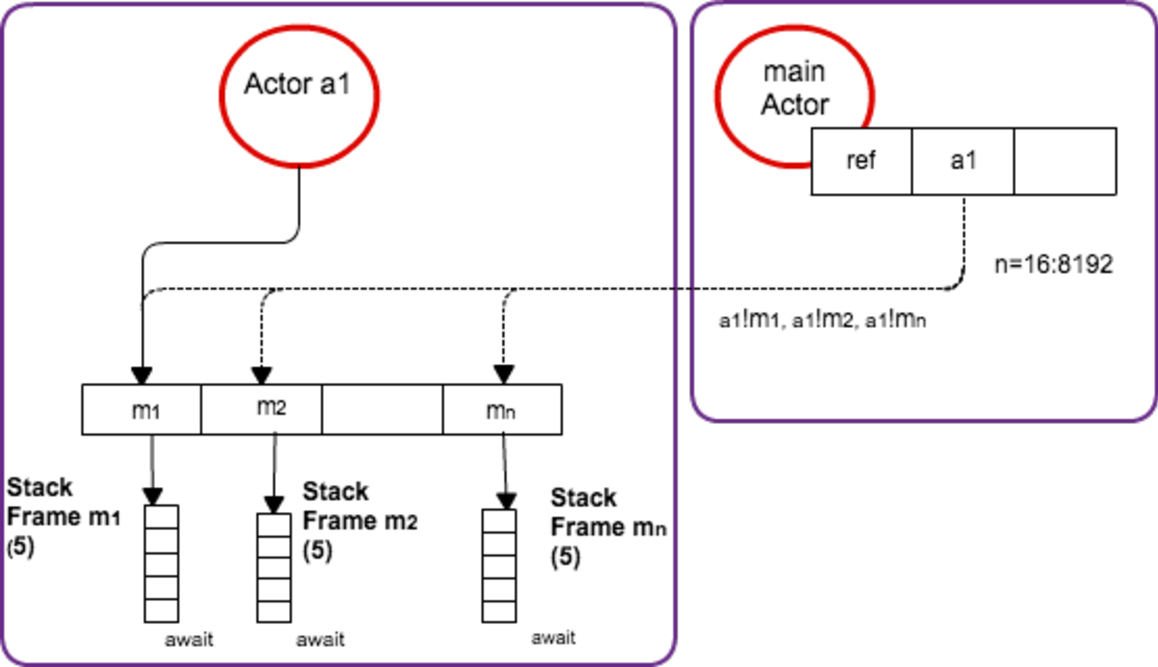
\includegraphics[scale=0.6]{scenario}
%	\caption{Cooperative Scheduling Benchmark Scenario}
%\end{figure}


\begin{lstlisting}[caption= Benchmark Example, label=absex]
module Recursive;

interface Ainterface {
	Int recursive_m(Int i, Int id);
}

class A() implements Ainterface{
	Int result=0;
	Int recursive_m(Int i, Int id){
		if (i>0){
			this.recursive_m(i - 1,id);	
		}
		else{
			Fut<Int> f = this ! compute( );
			await f ?;
		}
		return 1;
	}
	Int compute( ){
		result = result + 1;	//no significant computation
		return result;
}	}

{ // Main block:
	Int i = 0;	
	Ainterface master = new A ( );
	List<Fut<Int>> futures = Nil;	
	while( i < 500){		
		Fut<Int> f = master ! recursive_m (5, i);
		futures = Cons( f, futures );
		i = i + 1 ;
	}
	while ( futures != Nil ){
		Fut<Int> f1 = head(futures);
		futures = tail(futures);
		Int r = f1.get;
}	}
\end{lstlisting}
 \par Essentially we want to benchmark the pure overhead that arises from having a runtime system with cooperative scheduling support, both in a data-oriented approach and a process-oriented approach. The results are shown in Figure \ref{jj}. The performance figures presented are for one actor that is running 500-2500 method invocations. It is important to observe that each invocation generates 2 messages in the actor's queue, so as the number of calls increases the number of messages doubly increases. The figures show that the trade-off for storing continuations into memory instead of saving them in native threads removes limitations on the application and significantly reduces overhead.
\begin{figure}
	\centering
	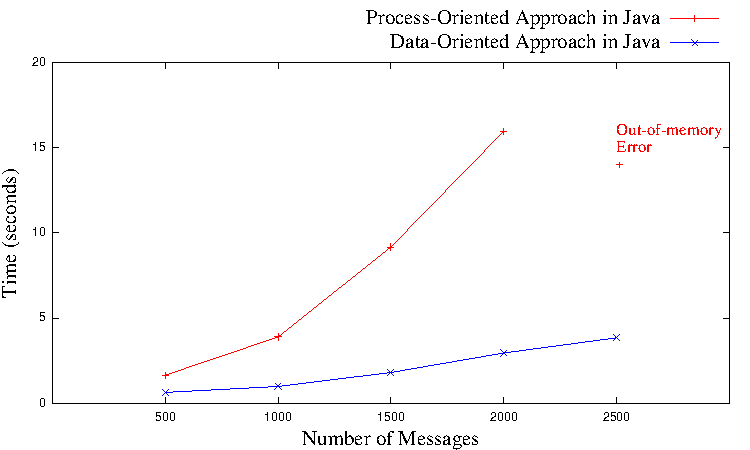
\includegraphics[scale=.9]{jaj8.pdf}
	\caption{Performance figures of the two Java implementations for Cooperative Scheduling}
	\label{jj}
\end{figure}

\par These results do show the drawback of native Java threads. However, while our solution is catered towards a widely-used software development language, it doesn't mean that there aren't other languages that are more suited to implement ABS language concepts efficiently using threads and without these limitations. In Section \ref{optimizations} we listed several optimizations that were inferred from our implementation solution. What we want to do is compare this optimized solution to an ABS backend implemented in Erlang that uses the same process-oriented approach but does not suffer from any limitation of native threads. We want to observe if our data-oriented approach can be comparable to Erlang's lightweight threads. The result in Figure \ref{ej} show that our approach fares better once the number of invocations passes 3000. This result also strengthens ABS purpose to provide a programming language for real applications.

\begin{figure}
	\centering
	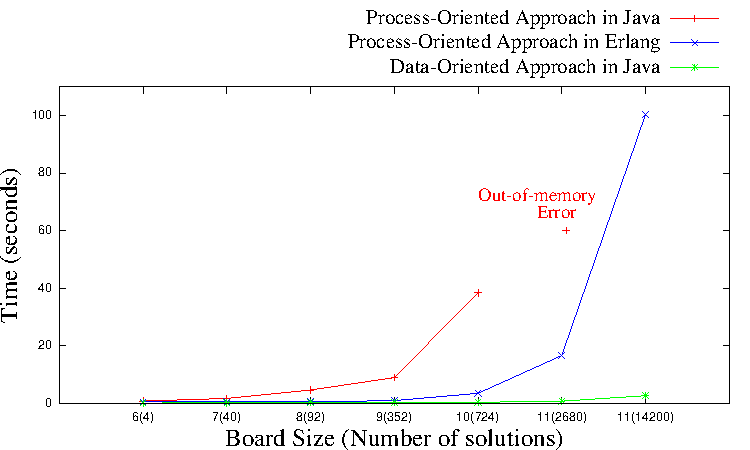
\includegraphics[scale=.9]{erlj8.pdf}
	\caption{Performance figures of the Erlang and Java backends for Cooperative Scheduling}
	\label{ej}
\end{figure}



